\section{XFS}
\subsection{Introducción}
\begin{frame}{Introducción}
  \begin{itemize}
    \item Creado por Silicon Graphics para IRIX.
    \item Liberado bajo licencia GPL en Mayo del 2000.
    \item Actualmente incluido en el kernel de Linux
    \item Opción en muchas distribuciones.
  \end{itemize}
\end{frame}

\subsection{Características}
\begin{frame}{Características}
  \begin{itemize}
    \item Journaling (Solo para los metadatos)
    \item ACLs
    \item Permisos POSIX
    \item Tamaño máximo: 9EB
    \item Tamaño máximo de fichero: 9EB
    \item Máximo de caracteres de nombre de fichero: 255B
    \item Máximo número de ficheros: NA
  \end{itemize}
\end{frame}

\subsection{Estructura}
\begin{frame}{Estructura}
  \begin{itemize}
    \item En XFS no existe el espacio para el sector de arranque.
    \item El espacio se divide completamente en “Grupos de Asignación”
    \item Cada grupo de asignación esta compuesto por:
    \begin{itemize}
      \item El superbloque (Si no es el primer grupo, solo es una copia).
      \item Un espacio para información de asignación de bloques e inodos del grupo (almacenada en arboles B+).
      \item Y un bloque de datos donde se almacenan los inodos y bloques de datos.
    \end{itemize}
  \end{itemize}
\end{frame}

\begin{frame}{Estructura}
  \begin{center}
    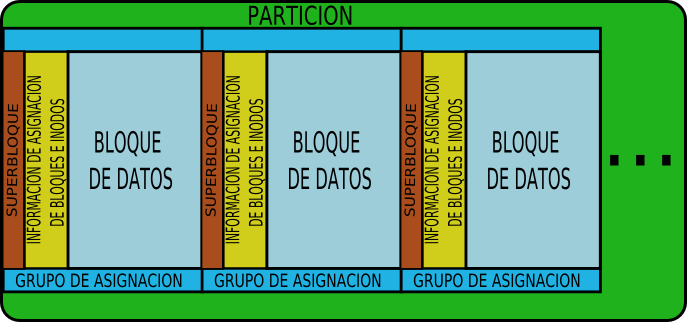
\includegraphics[height=5.5cm]{imgs/xfs_struct.png}
  \end{center}
\end{frame}

\begin{frame}{Ficheros}
  \begin{itemize}
    \item Los inodos contienen un núcleo con la información básica.
    \item Para especificar los bloques de datos usa “extents”, es decir, dirección inicial y tamaño total.
    \item Los inodos pueden tener almacenar los datos del fichero de tres maneras:
    \begin{itemize}
      \item NULO: No hay ningún dato, por lo tanto no hay extents.
      \item EXTENTS: Un mapa de extents de bloques de datos.
      \item B+ EXTENTS: Un árbol B+ de extents en el que los nodos hoja son bloques de datos.
    \end{itemize}
  \end{itemize}
\end{frame}

\begin{frame}{Ficheros}
  \begin{center}
    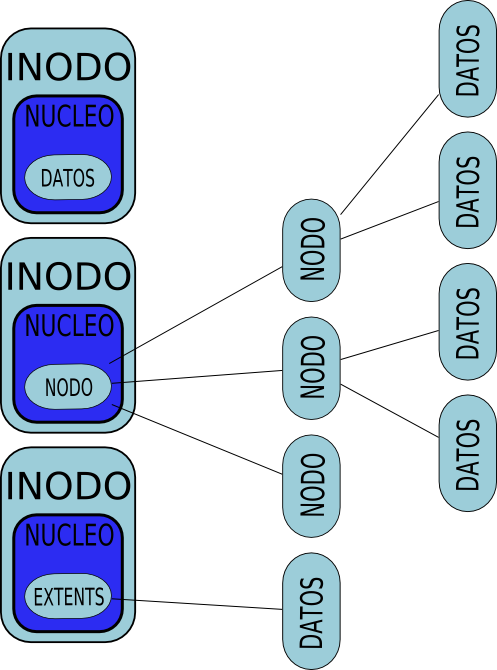
\includegraphics[height=6cm]{imgs/xfs_files.png}
  \end{center}
\end{frame}
